\documentclass{article}
\usepackage[a4paper]{geometry}
\usepackage{tikz}
\usepackage{pgfplots}
\pgfplotsset{compat=1.18}

\begin{document}

\title{just some graph tests, with pdfplots which uses tikz it seems like}
\author{daniel}
\maketitle



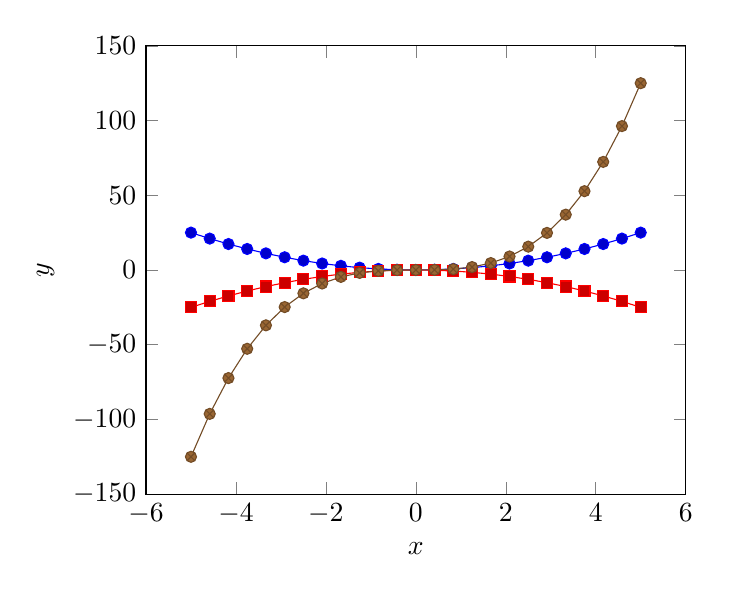
\begin{tikzpicture}
	\begin{axis}
		[xlabel= $x$, ylabel= $y$]
	\addplot{x^2};
	\addplot{-x^2};
	\addplot{x^3};
	\end{axis}
\end{tikzpicture}\\
Above are: $x^2, -x^2 and x^3$

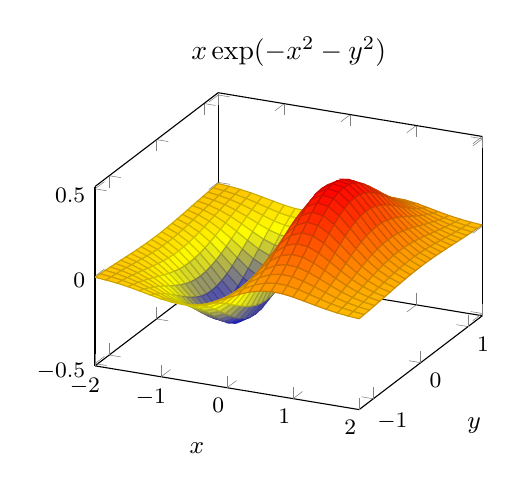
\begin{tikzpicture} \begin{axis}[
    title={$x \exp(-x^2-y^2)$},
    xlabel=$x$, ylabel=$y$,
    small,
]
\addplot3 [
        surf,
        domain=-2:2,
        domain y=-1.3:1.3,
    ] {exp(-x^2-y^2)*x};
\end{axis}
\end{tikzpicture}

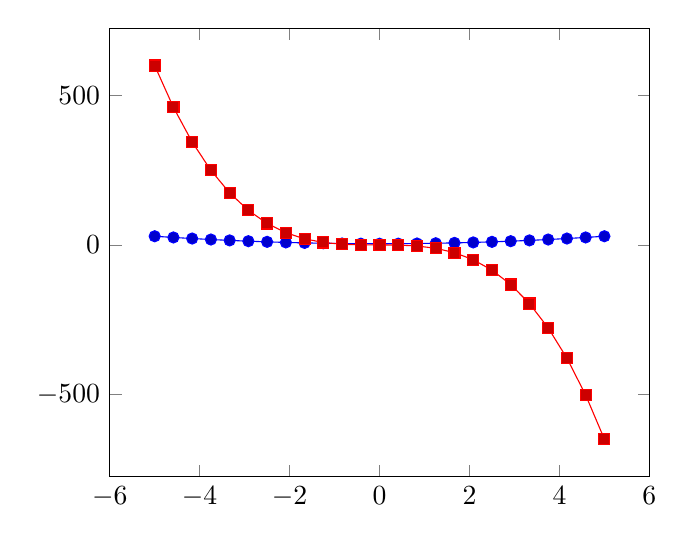
\begin{tikzpicture}
\begin{axis}
 \addplot{x^2 + 4};
 \addplot{-5*x^3-x^2};

\end{axis}
\end{tikzpicture}


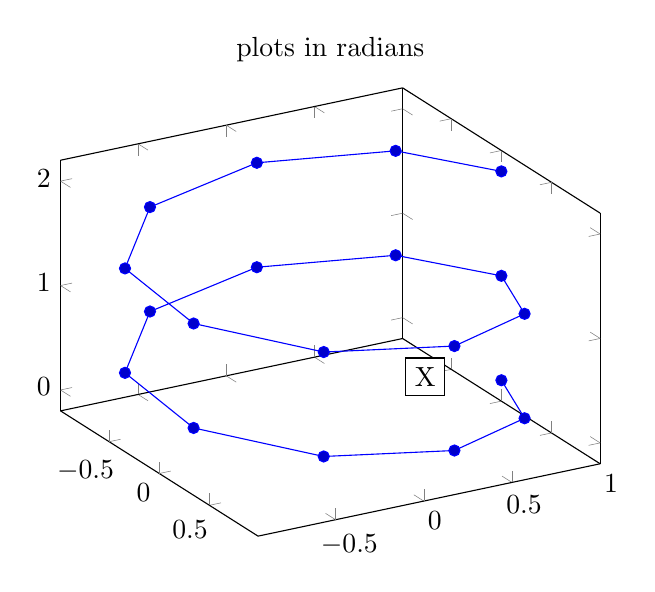
\begin{tikzpicture} \begin{axis}[view={60}{30},trig format plots=rad,
    title=plots in radians,
]
    \addplot3+ [domain=0:4*pi,samples=19,samples y=1]
        ({sin(x)},
         {cos(x)},
         {2*x/(4*pi)});
    % drawing instructions still use PGF's default
    \node [fill=white,draw=black,anchor=center] at
        ({sin(90)},{cos(90)},1) {X};
\end{axis}
\end{tikzpicture}


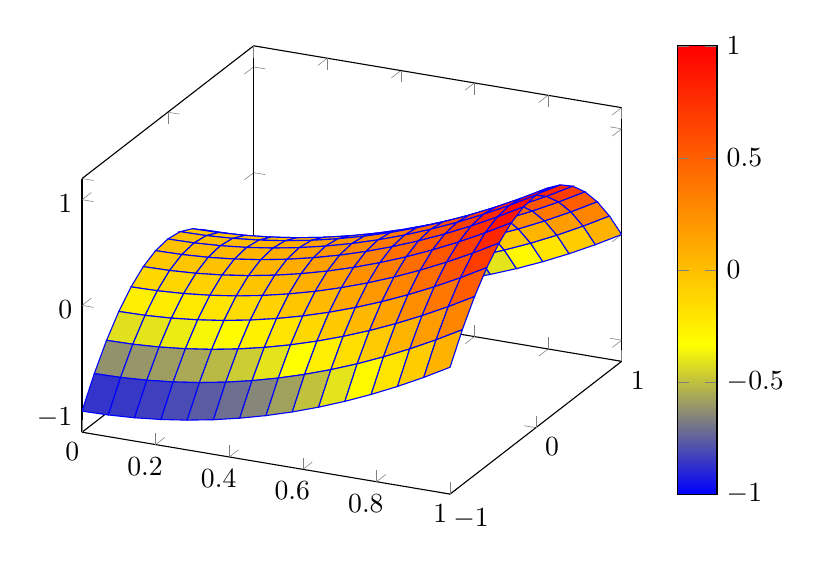
\begin{tikzpicture} \begin{axis}[colorbar]
    \addplot3 [
        surf,
        faceted color=blue,
        samples=15,
        domain=0:1,y domain=-1:1
    ] {x^2 - y^2};
\end{axis}
\end{tikzpicture}

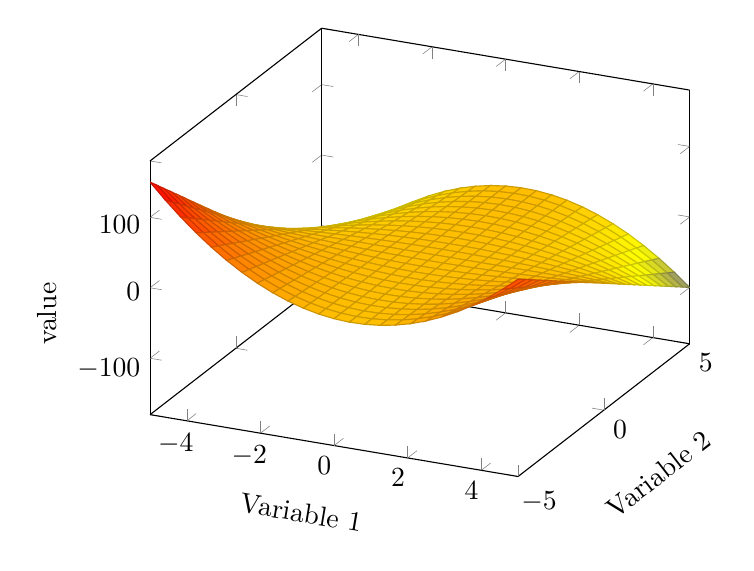
\begin{tikzpicture} \begin{axis}[
    xlabel=Variable 1,
    ylabel=Variable 2,
    zlabel=value,
    xlabel style={sloped like x axis},
    ylabel style={sloped},
]
    \addplot3 [surf] {y*x*(1-x)};
\end{axis}
\end{tikzpicture}

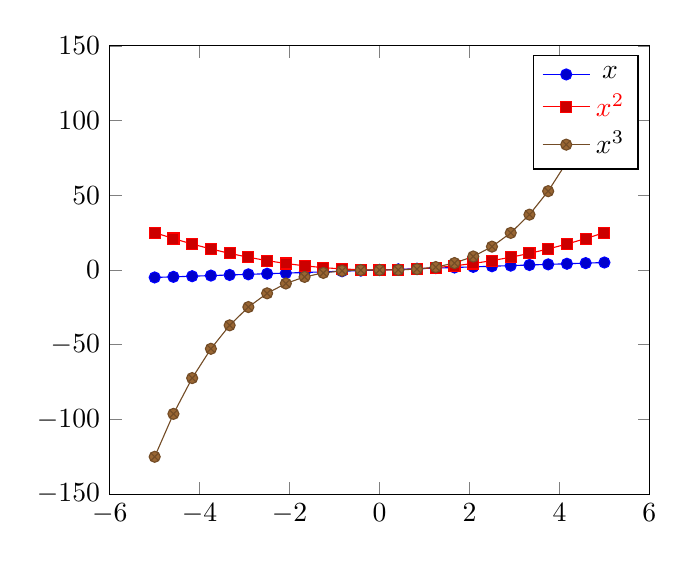
\begin{tikzpicture} \begin{axis}[
    legend entries={$x$,[red]$x^2$,$x^3$},
]
    \addplot {x};
    \addplot {x^2};
    \addplot {x^3};
\end{axis}
\end{tikzpicture}

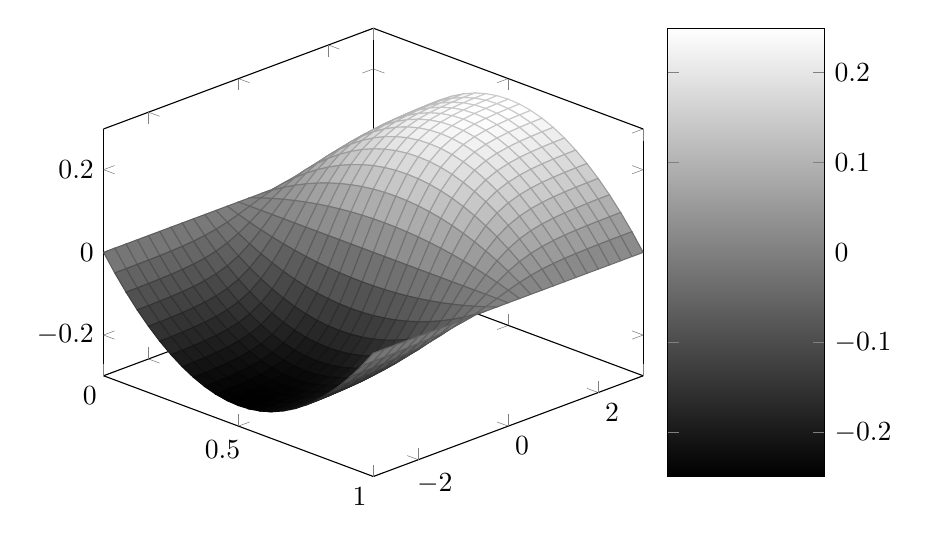
\begin{tikzpicture}
    \begin{axis}[
        view/az=45,
        colorbar,
        colorbar/width=2cm,
        colormap/blackwhite,
    ]
        \addplot3 [surf,domain=0:1,y domain=-3:3] {x*(1-x)*tanh(y)};
    \end{axis}
\end{tikzpicture}


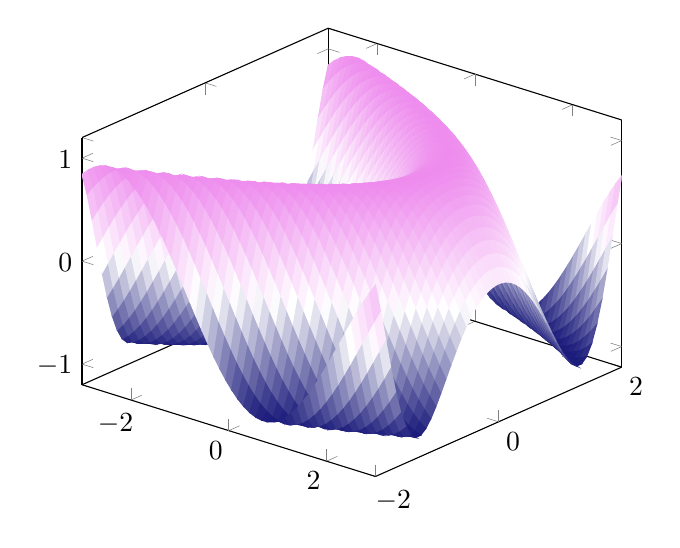
\begin{tikzpicture} \begin{axis}[view/h=40,colormap/violet]
    \addplot3 [
        surf,
        %shader=interp,
        shader=flat,
        samples=50,
        domain=-3:3,y domain=-2:2,
    ]
        {sin(deg(x+y^2))};
\end{axis}
\end{tikzpicture}


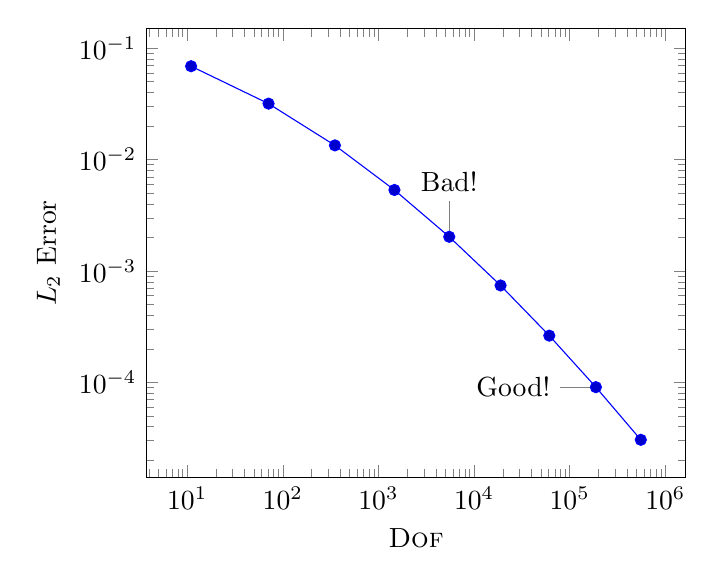
\begin{tikzpicture}
\begin{loglogaxis}[
    xlabel={\textsc{Dof}},
    ylabel={$L_2$ Error},
]
    \addplot coordinates {
        (11,     6.887e-02)
        (71,     3.177e-02)
        (351,    1.341e-02)
        (1471,   5.334e-03)
        (5503,   2.027e-03)
        (18943,  7.415e-04)
        (61183,  2.628e-04)
        (187903, 9.063e-05)
        (553983, 3.053e-05)
};
    \node [coordinate,pin=above:{Bad!}]
        at (axis cs:5503,2.027e-03)   {};
    \node [coordinate,pin=left:{Good!}]
        at (axis cs:187903,9.063e-05) {};
    \end{loglogaxis}
\end{tikzpicture}




\end{document}
